\documentclass[../dissertation.tex]{subfiles}
\begin{document}

\chapter{Review of the Field}

\section{Data Visualisation}

The visualisation of data is a field of critical importance that many huge companies rely on in order to make predictions, improve themselves, and get an edge over competitors. Data Visualisation is ``the presentation of data in a pictorial or graphical format [which] enables decision makers to see analytics presented visually, so they can grasp difficult concepts or identify new patterns.'' \cite{sasdv}, as defined by SAS - a world leader in the field. This clearly defines Data Visualisation and how it is useful.

Visualisation of data can be static or interactive, with interactive visualisations able to give a user more information. This can be done by: letting a user select part of a visualisation and hence gain a greater understanding of the data, changing parameters for the visualisation and observing changes, or the moving of nodes in a network and seeing how the rest of the network responds. This can greatly improve the usefulness of the visualisation for users, with new trends or vulnerabilities becoming clearer faster through interacting with the visualisation. Theus stated that, ``Interactive statistical data visualization is a powerful tool which reaches beyond the limits of static graphs'' \cite{theus2002interactive}.

\section{Network Visualisation}

Network Visualisation is a branch of Data Visualisation involving the ability to display nodes and edges in a meaningful way to a user. Nodes can represent any object, from people to countries to laws, and edges are used to display when there is a connection between two nodes. This can be used for a large variety of purposes, such as to ``identify nodes with the most links, nodes straddling different subgroups, and nodes isolated by their lack of connections'' \cite{flowingdata}. All of these tasks would be far more difficult without network visualisation.

\section{Visualisation of Massive Networks}

Visualisation of massive networks can lead to many challenges. Massive is a very vague term, but is generally considered as anything above about a thousand nodes \cite{batagelj1998pajek}. These challenges generally present themselves in the form of computational challenges or visualisation challenges. Computational challenges are when a system struggles to display a network visualisation due to lack of speed or performance from the CPU, RAM or backing storage. If a machine has a slow processor then the amount of time to create and then render the network will be increased greatly. Similarly, ``data sets are often too massive to fit completely inside the computer's internal memory'' \cite{abello2013handbook}. If the RAM is not big enough to fit the network, then the performance of the network visualisation will degrade significantly due to external memory needing to be used. 

The other computational challenge is the ability to store the network. Normally data is stored locally on a machine and loaded into a system in order to visualise it. However, when storing multiple massive networks, it can be nearly impossible to store this data on one machine. Hence, storing data on the cloud is often turned to, whether internally hosted within a company or externally hosted. This has a benefit as ``Cloud computing is a powerful technology to perform massive-scale and complex computing.'' \cite{hashem2015rise}, meaning that huge amounts of data can be efficiently stored and processed.

Assuming that the machine is powerful enough in all of the above ways, and is capable of visualising massive networks, the next challenge is how to present that data in any meaningful way. When visualising a few hundred or thousand nodes, it is generally fairly easy to get useful information out of the visualisation. However, when a user is faced with a few hundred thousand nodes or even several million, it can be very difficult to gain any sort of insight from the visualisation. 

\section{Visualisation of Massive Networks in a Browser}

Visualising massive networks in a browser adds several more constraints. Firstly, it requires all data to be sent over the internet so high bandwidth is required and even then, depending on the network size, a huge amount of time could be taken waiting for the network to download. Secondly, it requires any client-side processing to be done in JavaScript, which means that all code is run on a single thread and hence performance is poor when working with large datasets. Furthermore, JavaScript is necessary in order to render the network which is, again, a very slow process for large amounts of information. 

A goal of the project was to research techniques currently used to visualise massive networks, look into how successful they were, and then make a system that allows for the visualisation of massive networks in a browser and across a network. 

\section{Example within the Field}

\subsection{Visual Investigator}

Currently, the SAS product Visual Investigator \cite{sasvi} lets users view a network of entities in the system to see how they connect (for example: names, phone numbers and addresses). This works perfectly for a few entities, with useful information being shown clearly. However, with potentially millions of nodes, the network no longer shows much useful or practical information - just a mass of nodes - and becomes unusably slow (Visual Investigator is a web app and both processing power and memory are hard limits which, depending on network size, will easily be hit). However, it is worth nothing that the 'mass of nodes' can still show useful information despite initially looking meaningless. The overall shape of the network can highlight bottlenecks of the system, or potential threats or holes in a system.

As can be seen in Figures \ref{fig:30nodes}, \ref{fig:1000nodes}, \ref{fig:2500nodes}, \ref{fig:7500nodes}, the network starts out clear and loading times are instant, but it soon becomes both difficult to understand and slow. The times shown in the below figures are from the initial release version of Visual Investigator, and since then performance has improved in many ways. However, if there was a way to both speed up the loading times of huge networks, and make them convey meaningful information to the user, this would be benefit the system greatly.

\begin{figure}
\centering
\begin{minipage}{.5\textwidth}
    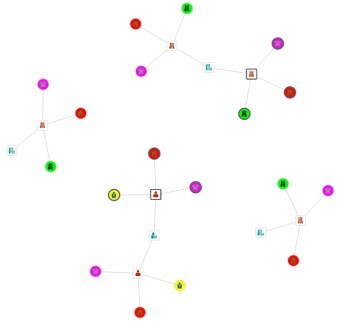
\includegraphics[width=\textwidth]{3/30_nodes}
    \caption{30 nodes, Loading Time less than 1 second}
    \label{fig:30nodes}
\end{minipage}%
\begin{minipage}{.5\textwidth}
    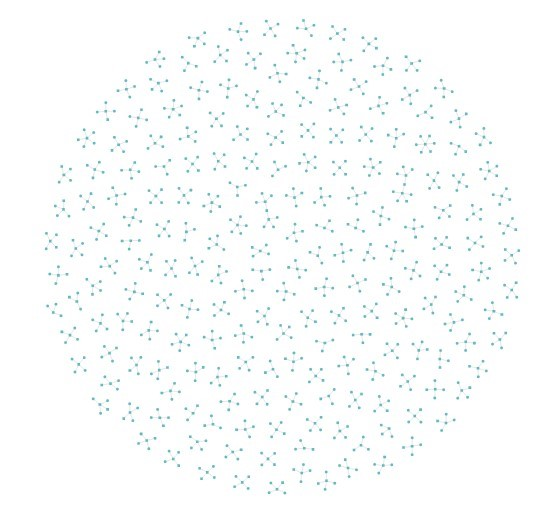
\includegraphics[width=\textwidth]{3/1000_nodes}
    \caption{1000 nodes, Loading Time 10 seconds}
    \label{fig:1000nodes}
\end{minipage}
\end{figure}

\begin{figure}
\centering
\begin{minipage}{.5\textwidth}
    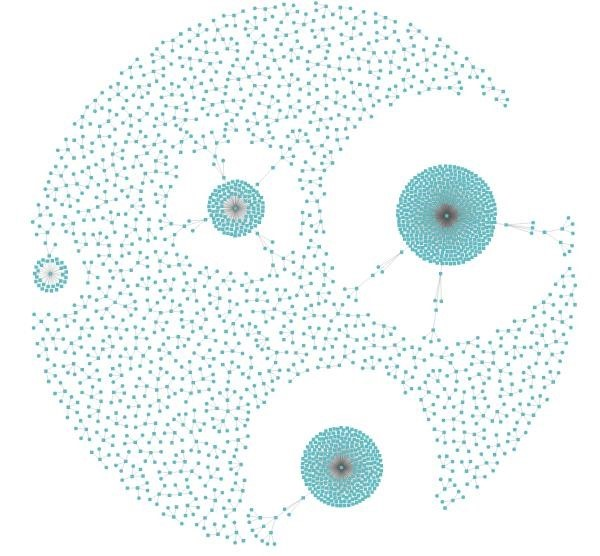
\includegraphics[width=\textwidth]{3/2500_nodes}
    \vspace*{3.5mm}
    \caption{2500 nodes, Loading Time 30 seconds}
    \label{fig:2500nodes}
\end{minipage}%
\begin{minipage}{.5\textwidth}
    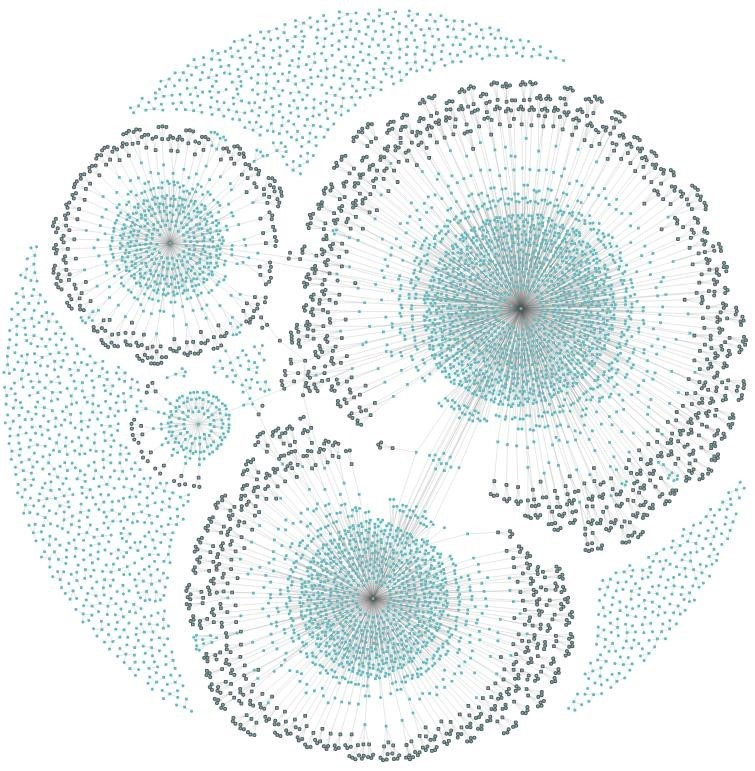
\includegraphics[width=\textwidth]{3/7500_nodes}
    \caption{7500 nodes, Loading Time 300 seconds}
    \label{fig:7500nodes}
\end{minipage}
\end{figure}

\end{document}